\documentclass[a4paper,11pt]{report}


%%%%%%%%%%%%%%%%%%%%%%%%%%%%
% University of Sussex thesis template
%%%%%%%%%%%%%%%%%%%%%%%%%%%%
% Modification History
%
% Based on usthesis.cls by Jonathon Read
% http://www.cogs.susx.ac.uk/users/jlr24/latex.html
% Modified by Anthony Smith, Feb 2007
% Incorporated into single thesis.tex file, Anthony Smith, 30 June 2008
% Minor alterations to page numbering, AJS, 25 July 2008
% New alternative hyperref options for print version, AJS, 11 Sep 2008
% "DRAFT" on header, AJS, 12 Sep 2008
%%%%%%%%%%%%%%%%%%%%%%%%%%%%


%%%%%%%%%%%%%%%%%%%%%%%%%%%%
% LINE SPACING
\newcommand{\linespacing}{1.5}
\renewcommand{\baselinestretch}{\linespacing}
%%%%%%%%%%%%%%%%%%%%%%%%%%%%


%%%%%%%%%%%%%%%%%%%%%%%%%%%%
% BIBLIOGRAPHY STYLE
\usepackage{natbib}
% \bibliographystyle{plain} for [1], [2] etc.
\bibliographystyle{apalike}
%%%%%%%%%%%%%%%%%%%%%%%%%%%%


%%%%%%%%%%%%%%%%%%%%%%%%%%%%
% OTHER FORMATTING/LAYOUT DECLARATIONS
% Graphics
\usepackage{graphicx,color}
\usepackage{epstopdf}
\usepackage[british]{babel}
% The left-hand-side should be 40mm.  The top and bottom margins should be
% 25mm deep.  The right hand margin should be 20mm.
\usepackage[a4paper,top=2.5cm,bottom=2.5cm,left=4cm,right=2cm,headsep=10pt]{geometry}
\flushbottom
% Pages should be numbered consecutively thorugh the main text.  Page numbers
% should be located centrally at the top of the page.
\usepackage{fancyhdr}
\fancypagestyle{plain}{
	\fancyhf{}
	% Add "DRAFT: <today's date>" to header (comment out the following to remove)
	\lhead{\textit{DRAFT: \today}}
	%
	\chead{\thepage}
	\renewcommand{\headrulewidth}{0pt}
}
\pagestyle{plain}
%%%%%%%%%%%%%%%%%%%%%%%%%%%%


%%%%%%%%%%%%%%%%%%%%%%%%%%%%
% ANY OTHER DECLARATIONS HERE:

\usepackage{amsmath} %Needed for typing equations and theorems
\usepackage{amssymb} %Loads additional fonts and symbols
\usepackage{graphicx} %Needed for adding graphics to the document
\usepackage{verbatim} %Needed for \verbatiminput
\usepackage{color}
%\usepackage{longtable} 
\usepackage{listings} 
\usepackage{float}
\usepackage{wrapfig} %http://en.wikibooks.org/wiki/LaTeX/Floats,_Figures_and_Captions

\newcommand{\bv}[1]{\mathbf{#1}}
\newcommand{\bhv}[1]{\mathbf{\hat{#1}}}
\newcommand{\M}[1]{\mathbf{#1}}
\newcommand{\defeq}{\stackrel{\text{\tiny def}}{=}}
\newcommand{\R}{\mathbb{R}}

\newcommand{\red}[1]{\color{red}#1\color{black}}
\newcommand{\blue}[1]{\color{blue}#1\color{black}}
\newcommand{\figtitle}[1]{\Large{#1} \vfill \vspace{15pt}}
%%%%%%%%%%%%%%%%%%%%%%%%%%%%


%%%%%%%%%%%%%%%%%%%%%%%%%%%%
% HYPERREF
\usepackage[colorlinks,pagebackref,pdfusetitle,urlcolor=blue,citecolor=blue,linkcolor=blue,bookmarksnumbered,plainpages=false]{hyperref}
% For print version, use this instead:
%\usepackage[pdfusetitle,bookmarksnumbered,plainpages=false]{hyperref}
%\usepackage{backref}
%\renewcommand{\backrefpagesname}{Cited on}
%%%%%%%%%%%%%%%%%%%%%%%%%%%%


%%%%%%%%%%%%%%%%%%%%%%%%%%%%
% BEGIN DOCUMENT
\begin{document}
%%%%%%%%%%%%%%%%%%%%%%%%%%%%


%%%%%%%%%%%%%%%%%%%%%%%%%%%%
% PREAMBLE: roman page numbering i, ii, iii, ...
\pagenumbering{roman}
%%%%%%%%%%%%%%%%%%%%%%%%%%%%


%%%%%%%%%%%%%%%%%%%%%%%%%%%%
%% TITLE PAGE: The title page should give the following information:
%%	(i) the full title of the thesis and the sub-title if any;
%%	(ii) the full name of the author;
%%	(iii) the qualification aimed for;
%%	(iv) the name of the University of Sussex;
%%	(v) the month and year of submission.
\thispagestyle{empty}
\begin{flushright}

\includegraphics[width=6cm]{fig/uslogo.pdf}
\end{flushright}	
\vskip40mm
\begin{center}
% TITLE
\huge\textbf{How Does Morphological Change Accelerate Evolution?}
\vskip2mm
% SUBTITLE (optional)
\LARGE\textit{Who knows?}
\vskip5mm
% AUTHOR
\Large\textbf{Shane Celis}
\normalsize
\end{center}
\vfill
\begin{flushleft}
\large
% QUALIFICATION
Submitted for the degree of Master of Science \\
University of Sussex	\\
% DATE OF SUBMISSION
September 2011
\end{flushleft}		
%%%%%%%%%%%%%%%%%%%%%%%%%%%%


%%%%%%%%%%%%%%%%%%%%%%%%%%%%
% DECLARATIONS
\chapter*{Declaration}
I hereby declare that this thesis has not been and will not be submitted in whole or in part to another University for the award of any other degree.
	
% ADDITIONAL DECLARATIONS HERE (IF ANY)

\vskip5mm
Signature:
\vskip20mm
% AUTHOR
Shane Celis
%%%%%%%%%%%%%%%%%%%%%%%%%%%%


%%%%%%%%%%%%%%%%%%%%%%%%%%%%
% SUMMARY PAGE
\thispagestyle{empty}
\newpage
\null\vskip10mm
\begin{center}
\large
\underline{UNIVERSITY OF SUSSEX}
\vskip20mm
% AUTHOR, QUALIFICATION
\textsc{Shane Celis, Master of Science}
\vskip20mm
% TITLE
\underline{\textsc{My Theory of Everything}}
\vskip0mm
% SUBTITLE (optional)
\underline{\textsc{How it all works}}
\vskip20mm
\underline{\textsc{Summary}}
\vskip2mm
\end{center}
% Change line spacing
\renewcommand{\baselinestretch}{1.0}
\small\normalsize
% SUMMARY HERE (300 word limit for most subjects):

%%%%%%%%%%%%%%%%%%%%%%%%%%%%


%%%%%%%%%%%%%%%%%%%%%%%%%%%%
% ACKNOWLEDGEMENTS
\chapter*{Acknowledgements}
\renewcommand{\baselinestretch}{\linespacing}
\small\normalsize
% ACKNOWLEDGEMENTS HERE:

%%%%%%%%%%%%%%%%%%%%%%%%%%%%


%%%%%%%%%%%%%%%%%%%%%%%%%%%%
% TABLE OF CONTENTS, LISTS OF TABLES & FIGURES
\newpage
\pdfbookmark[0]{Contents}{contents_bookmark}
\tableofcontents
\listoftables
\phantomsection
\addcontentsline{toc}{chapter}{List of Tables}
\listoffigures
\phantomsection
\addcontentsline{toc}{chapter}{List of Figures}
%%%%%%%%%%%%%%%%%%%%%%%%%%%%


%%%%%%%%%%%%%%%%%%%%%%%%%%%%
% MAIN THESIS TEXT: arabic page numbering 1, 2, 3, ...
\newpage
\pagenumbering{arabic}
%%%%%%%%%%%%%%%%%%%%%%%%%%%%


%-----------------------------------------------------
% Chapter: Introduction
%-----------------------------------------------------

% NB Good idea to put each chapter in a separate file.
% If you put the following in a file called "thesis_introduction.tex"
% then you can include it with the following:

% \input{thesis_introduction}

\chapter{Introduction}
\label{chap:intro}

\chapter{Introduction}

Morphological change has been demonstrated to accelerate evolution of
robust behaviour in one instance. However, it is unclear how or why
this happens. This project evolves a robot with varying degrees of
conservation between the earlier and later forms to help answer the
question, under what conditions does morphological change accelerate
evolution?  Introduction Bongard showed the evolution of light
following behaviour was accelerated for robots that grew from a
leg-less anguilliform to a legged hexapod when compared to evolving a
hexapod with no morphological change [1]. This project is a critical
replication of that experiment.


\begin{comment}
  mention Minimal Simulation guy
  
  conventions bold denotes a vector
  hat means its a unit vector
  
\end{comment}

\chapter{Method}

This experiment uses a two-dimensional, aquatic-like environment to
test what kinds of morphological changes may accelerate evolution. The
morphological forms---inspired by frog metamorphosis---have been
selected such that the conservation of the infant form to the adult
form may be varied. Figure~\ref{morphology} shows the two principle
forms which may be parametrically varied by two variables $l_t, l_f
\in [0, 1]$ tail length and foot length respectively.  The full range
of morphological change will be described in detail in
section~\ref{morph-change}.  In the inspiring case, the individual
begins as a ``tadpole'' bearing only a tail. It transforms into a
``frog'' with four limbs. Its task is to swim to a target.

%\begin{wrapfigure}{r}{0.5\textwidth}
\begin{figure}[h]
  \centering
  \figtitle{Body Plans} 
  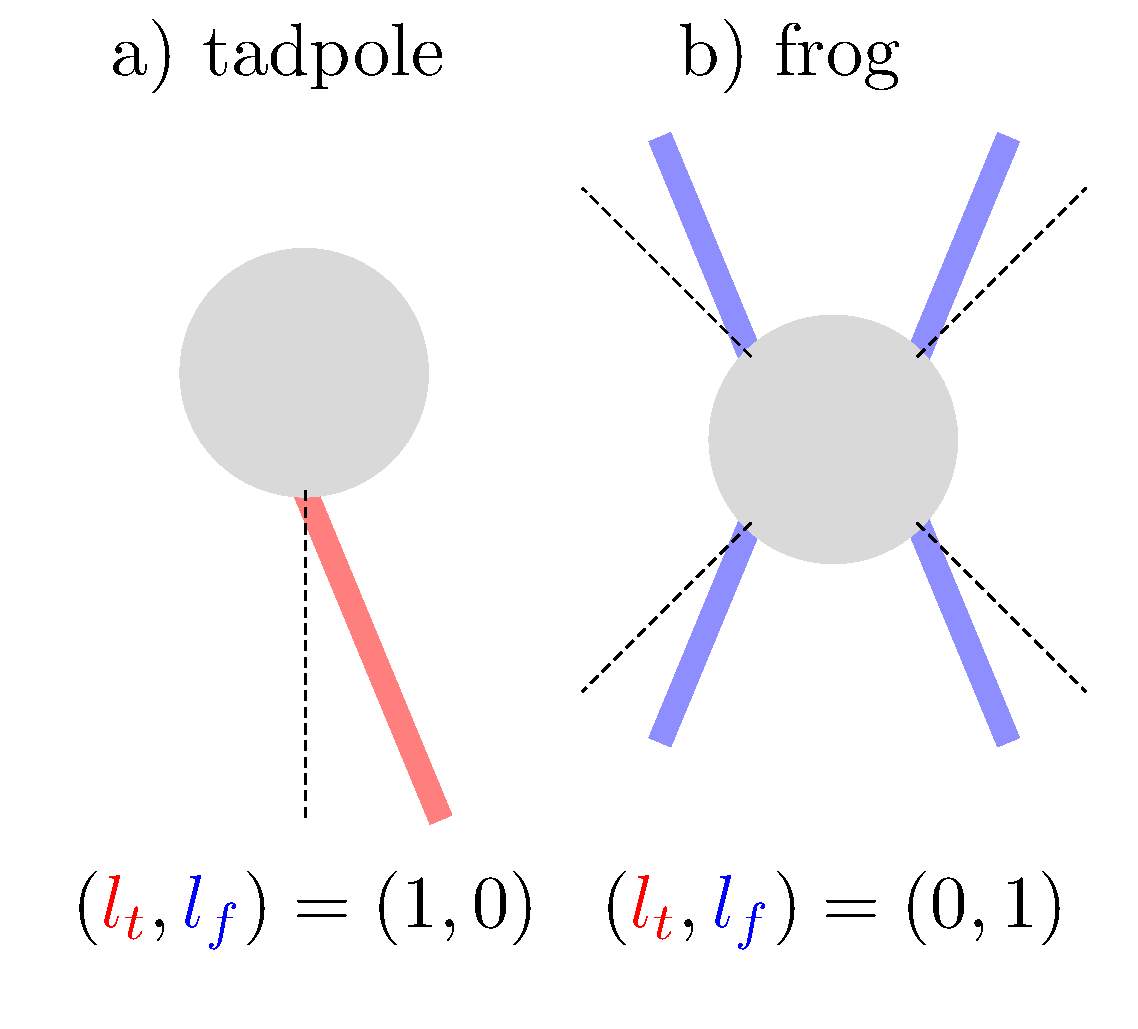
\includegraphics[scale=0.4]{fig/forms.pdf} 
  \vspace{-30pt}
  \caption[Body plans]{\label{morphology}Body plans parameterised by
    tail length $l_t$ and foot length $l_f$. a) represents the infant
    ``tadpole'' form, and b) represents the adult ``frog'' form. }
\end{figure}
%\end{wrapfigure}

\section{Physics Model}

This experiment uses the following physical model to simulate an
individual in an two-dimensional aquatic environment.  The aim of the
simulation is to provide a water-like environment, but it is not
intended to provide a realistic environment such that a controller
evolved in simulation could be easily transferred to a real robot.  It
is thought, however, that applying the same method with a real robot
would produce comparable results.

The virtual robot is composed of six rigid bodies: one central body,
one tail segment, and four feet segments.  The tail and feet are
connected to the central body by pinwheel joints.  Eight configuration
variables $\{q_1, q_2, \ldots, q_8\}$ describe the body as shown in
Figure~\ref{confvars}.  The position of the body is denoted by the
vector $(q_1, q_2)$.  The angle of the central body measured
counter-clockwise to the $\bf \hat j$ axis denoted by $q_3$.  The
angle of the tail and four feet are denoted by $q_4, \ldots, q_8$,
respectively.  Eight corresponding motion variables $\{u_1, u_2,
\ldots, u_8\}$ describe the generalised speeds of the body $u_i =
\frac{d q_i}{d t}$.

\begin{figure}  
  \centering
  \figtitle{Diagram of Configuration Variables} 
  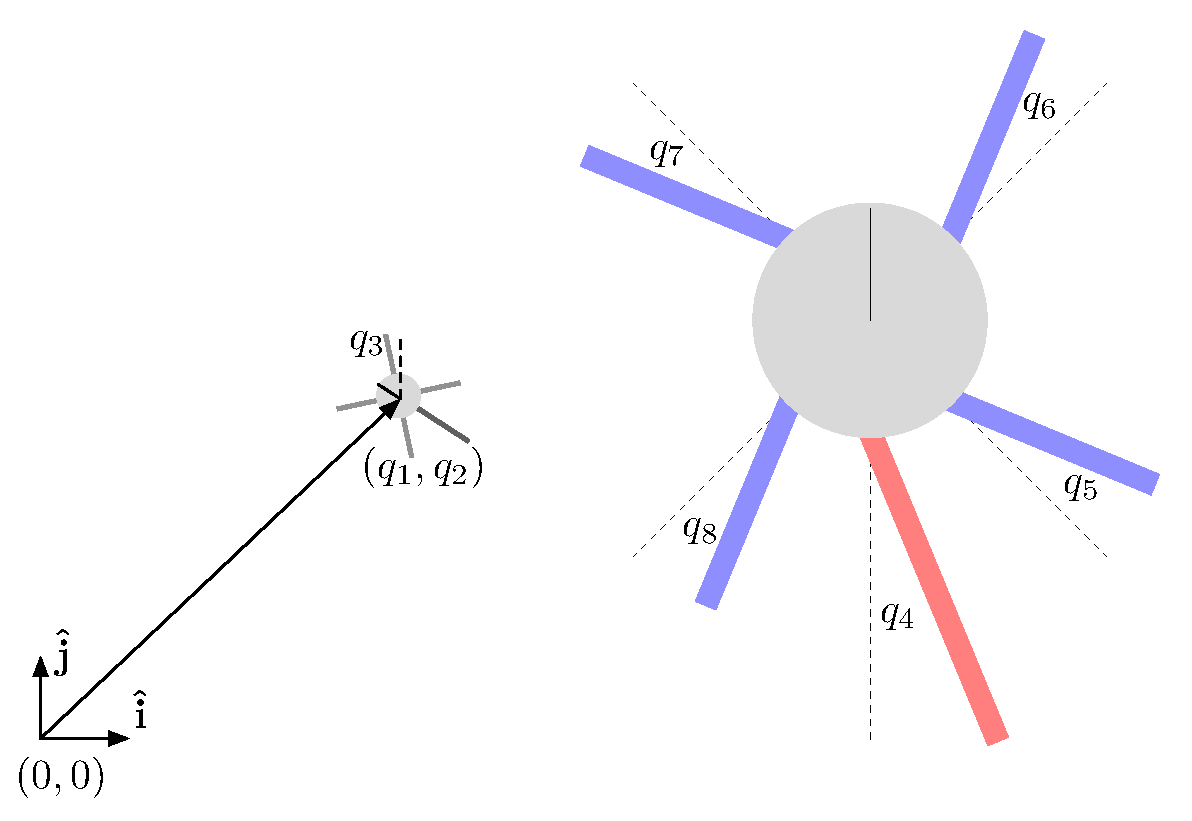
\includegraphics[scale=0.6]{fig/confvars.pdf} 
  \caption[Diagram of configuration variables]{\label{confvars}Diagram
    of the configuration variables $\{q_1, q_2, \ldots, q_8\}$ that
    fully describe the physical state of the body at time $t$}
\end{figure}

\section{Forces}

For each limb a drag force $\bv F_D$ opposes its direction of motion
which are given by Equation~\ref{drag-force-eq} where $\rho$ is the
density of the fluid, $c_d$ is the drag coefficient, $l$ is the length
of the limb, $w$ is the width of the limb, $\bhv n$ is the normal of
the limb, $\bv v_b$ is the velocity of the center of mass of the limb,
$\bv v_c$ is the velocity of the current, $\bv v$ is the relative
velocity of the limb with respect to the current, $A$ is the reference
area---an orthographic projection of the limb shape on a plane
perpendicular to the direction of motion.  Figure~\ref{drag-force}
shows these values for a limb.  The shape of the limb is taken to be a
rod of length $l$, width $w$, and depth $d$.  However, for the
purposes of computing the drag force, the width of the limb $w$ is set
to zero since $w \ll l$ and the force it might contribute is not
considered significant.

\begin{eqnarray}
  A &=& l\,d~ |\bhv v \cdot \bhv n| + l\, w~|\bhv v \times \bhv n|\\
  w &=& 0 \\
  \bv v &=& \bv v_b - \bv v_c \\
  \bv F_D &=& -\frac{1}{2} \rho\,c_d~||\bv v||^2\,A~\bhv v \\
  \bv F_D &=& -\frac{1}{2} \rho\, c_d~ l\,d~|\bv v \cdot \bhv n|\bv v \label{drag-force-eq} 
\end{eqnarray}


\begin{figure}[h]  
  \centering
  \figtitle{Diagram of Drag Force} 
  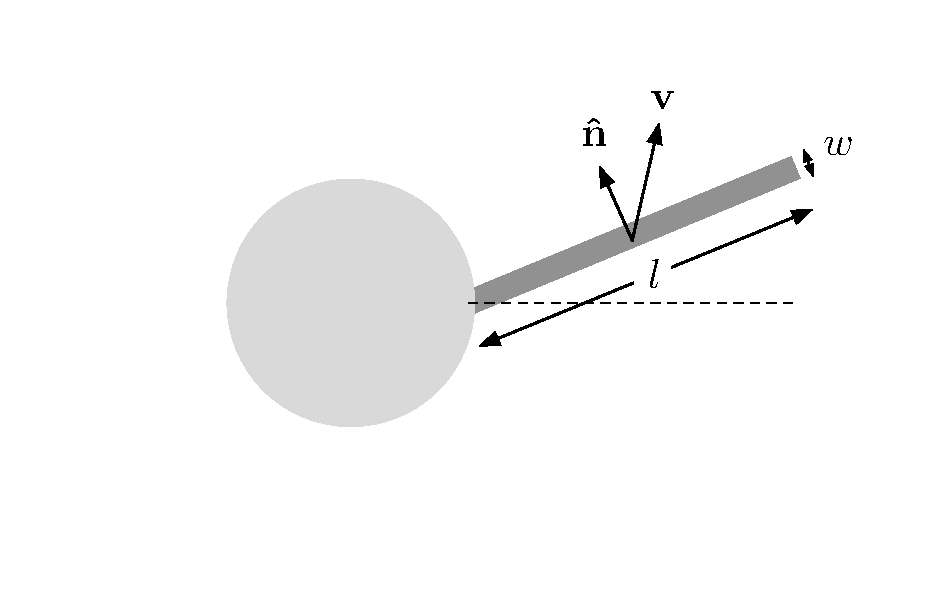
\includegraphics[scale=0.7]{fig/drag-force.pdf} 
  \vspace{-45pt}
  \caption[Diagram of drag force]{\label{drag-force}For each limb the
    length $l$, width $w$, depth $d$ (not shown), velocity of limb
    $\bv v_b $, velocity of current $\bv v_c$,, normal vector $\bhv n$
    determine its drag force $\bv F_D$.}
\end{figure}

In addition, a drag force and drag torque is exerted on the central
body.  The full equations of motion are given in the
Appendix~\ref{app:physeqns}.

\subsection{Collisions}

Interbody collisions are permitted, so limbs may freely move through
one another.\footnote{This is not thought objectionable because one
  can imagine constructing a robot with limbs arranged on planes such
  that they could pass each other unobstructed.}  However, the limbs
are constrained to not penetrate the central body.  When the angle of
a limb reaches $|q| = \frac{\pi}{2}$, a torque $T_c(q)$ is applied to
oppose further motion, shown in Equation~\ref{limb-bounded}.

\begin{eqnarray}
  T_c(q_{i}) &=& T_{max}~\bound(q_{i}, (\frac{- \pi}{2}, \frac{\pi}{2})) \text{ for } i \in [4,8] \label{limb-bounded} \\
  \bound(x, (a,b)) &=& \begin{cases}
    -1 & a \ge x \wedge b > x \\ 
    1 & a < x \wedge b \le x \\
    0 & \text{otherwise}
  \end{cases}
\end{eqnarray}


\section{Controller}

The controller used for the robot is a Continuous Time Recurrent
Neural Network (CTRNN).  The dynamics of a neuron $y_i$ is given by
Equation~\ref{ctrnn-eq} with time constant $\tau_i \in [0.1, 100]$,
weights $w_{ji} \in [-4, 4]$, bias $\theta_i \in [-2, 2]$, sensors
$s_j \in \R $, and sensor weights $n_{ji} \in [-4, 4]$.

\begin{eqnarray}
  \tau_i \frac{d y_i}{dt} &=& -y_i + \sum_{j = 1}^m w_{ji} \sigma(y_j - \theta_i) + \sum_{j=1}^s n_{ji} s_j \text{ for } i \in [1,5] \label{ctrnn-eq} \\
  \sigma(x) &=& \frac{1}{1 + e^{-x}}
\end{eqnarray}

\begin{table}
  \begin{center}
    \begin{tabular}{ | l | c | l | }
      \hline
      Sensor Variable & Value & Description \\
      \hline
      $s_1$ & $||(u_1, u_2) - (w_1, w_2)||$ & relative translational speed \\
      $s_2$ & $u_3$ & angular speed \\
      $s_3$ & $||target - (q_1, q_2)||$ & distance to target \\ 
      $s_4$ & $target_\theta$ & angle to target \\              
      $s_5$ & $q_4$ & position of tail \\                       
      $s_6$ & $u_4$ & speed of tail \\                          
      $s_{7 + 2 i}$ & $q_{5 + i}$ & position of each foot $i \in [0, 3]$ \\        
      $s_{8 + 2 i}$ & $u_{5 + i}$ & speed of each foot $i \in [0, 3]$ \\           
      \hline
    \end{tabular}
  \end{center}
  \caption[Sensors]{\label{table:sensor}Description of available sensors}
\end{table}

Table~\ref{table:sensor} describes the sensors.  A range finder for a
target is given by the $s_3$ and $s_4$ sensors.  Proprioceptive
sesnsors are given by the $s_5, s_6, \ldots, s_{14}$ sensors.  Five
motor neurons are used with weighted inputs from all sensors.  Each
neuron exerts a torque on an associated limb.  The torque for each
limb $T(q_i)$ is given in Equation~\ref{limb-torque}.

\begin{eqnarray}
  T(q_{i + 3}) &=& T_{max}~\clip(y_i) + T_c(q_{i + 3}) \text{ for } i \in [1,5] \label{limb-torque} \\
  \clip(x) &=& \begin{cases}
              1 & x > 1 \\
              -1 & x < -1 \\
              x & \text{otherwise} 
              \end{cases} 
\end{eqnarray}

\section{Genetic Encoding}

The CTRNN controller is specified by a real vector gene $\bv g \in [0,
  1]^{105}$.  Each gene component $g_k$ is associated with one and
only one of the CTRNN parameters $\tau_i, w_{ji}, \theta_i, \text{ and
} n_{ji}$.  The $w_{ji}, \theta_i,$ and $ n_{ji}$ parameters are
linearly mapped from the domain of the gene $[0,1]$ to the domain of
each parameter.  The $\tau$ parameter uses a non-linear mapping
$\tau_i = 10^{-2 + 4 g_k}$.

\section{Morphological Change}\label{morph-change}

Morphological change is considered over phylogenetic and ontogenetic
time.  Two adult forms are evolved: A) frog with a tail $({l_t},
{l_f}) = (1,1).$ B) frog without a tail $({l_t}, {l_f}) =
(0,1).$ The control case is no morphological change denoted $An$ and
$Bn$.  The first experimental cases concern phylogenetic change
denoted $Ap$ and $Bp$, which are divided into phases $p_i$.  The
second experimental case concerns ontogenetic change denoted $Ao$ and
$Bo$.  Figure~\ref{morph-regiment} shows the tail length ${l_t}$ in
red and feet length ${l_f}$ in blue for each experimental case.
The exact values used are recorded in the
Appendix~\ref{morph-regiment-values}.

\begin{figure}
  \centering
  \figtitle{Variations of Morphological Change} 
  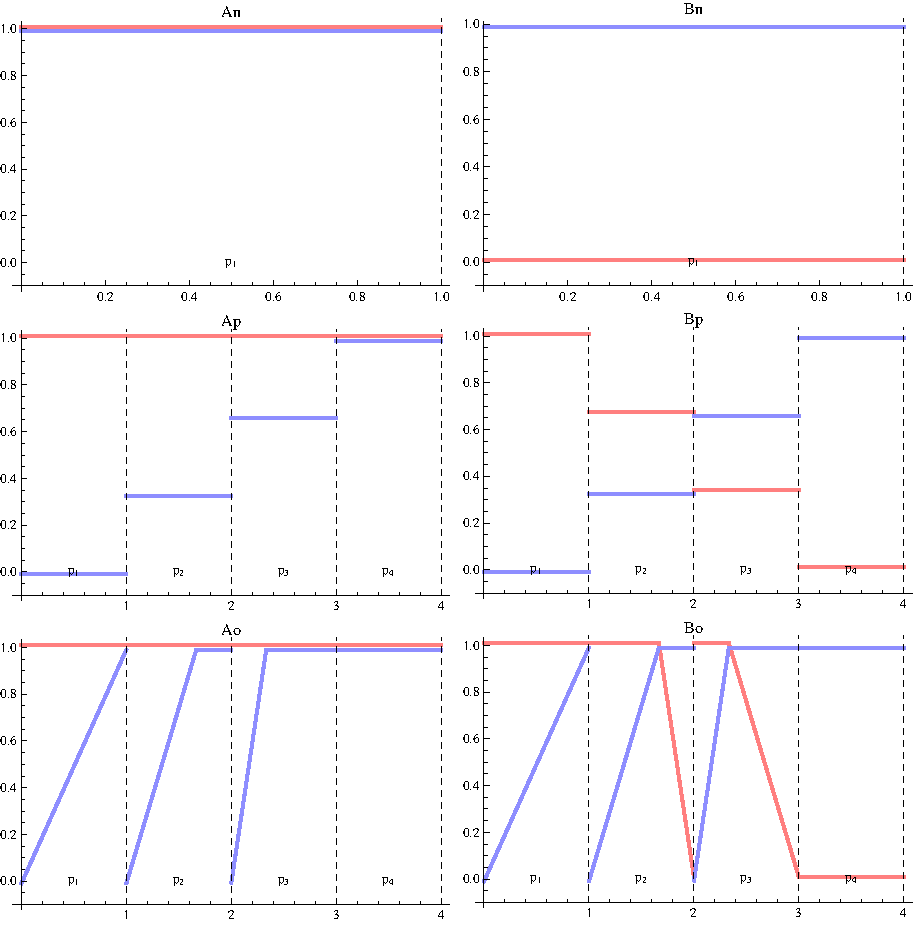
\includegraphics[scale=1.0]{fig/morph-regiment.pdf} 
  \vspace{-15pt}
  \caption[Variations of morphological
    change]{\label{morph-regiment}An, Bn do not change morphology;
    Ap, Bp change morphology over phylogenetic time; Ao, Bo change
    morphology over ontogenetic and phylogenetic time.}

\end{figure}

\section{Controller Variation}

In the test cases $Bp$ and $Bo$ the infant form is not conserved in
the adult form.  However, the controller may conserve some behaviour
acquired in the infant form that is useful in the adult form, which
may accelerate evolution.  To determine whether this happens, two
types of CTRNN controllers are considered: 1) a ``lobotomised''
controller, which has two independent CTRNNs, one for the tail; one
for the feet. 2) a ``non-lobotomised'' controller, which has one CTRNN
that controls both the tail and feet.  These are shown in
Figure~\ref{ctrnn-figures}.

\begin{figure}[h]
  \centering
  \figtitle{Variation of CTRNN Controllers} 
  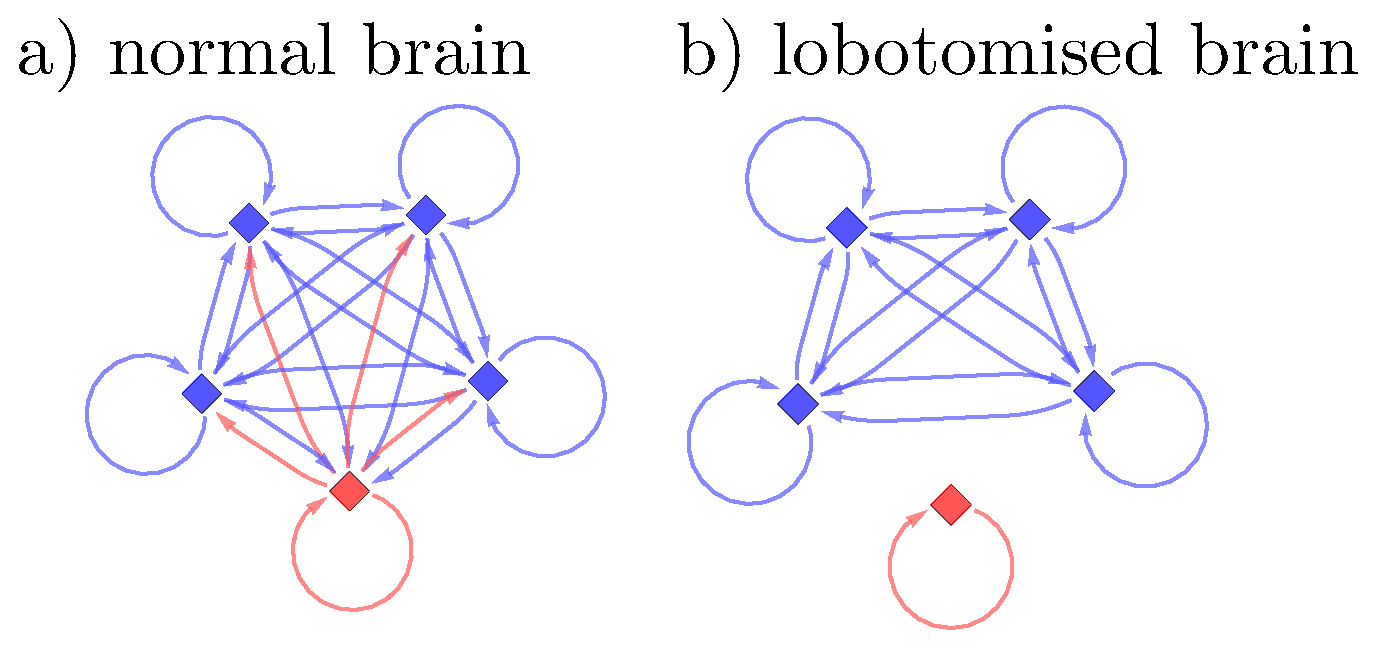
\includegraphics[width=5in]{fig/ctrnn-figures.pdf}
  \vspace{-15pt}
  \caption[Variation of CTRNN controllers]{\label{ctrnn-figures}a)
    Fully connected CTRNN controller. b) Independent CTRNN controllers
    for the tail and legs.}
\end{figure}

The sensors are altered for the ``lobotomised'' controller.  The tail
brain does not receive proprioceptive sensors from the other limbs
$\{s_7, s_8, \ldots, s_14\}$.  Likewise, the foot brain does not
receive proprioceptive sensors from the tail $s_5$ and $s_6$.
Otherwise, the sensors are the same.\footnote{Note on implementation:
  the ``lobotomised'' controller code is the same as the
  ``non-lobotomised'' with a specific set of weights $w_{ji}$ and
  sensor coefficients $n_{ji}$ set to zero.}

\section{Tasks}

To confirm the results are not spurious or a special case for one
particular task, multiple tasks of varying difficulty are considered.
The basic task is locomotion to a target.  Changing the target
location was considered, but it is hard to ascertain what positions of
the target would be more difficult.  The infant ``tadpole'' form with
its tail directed to the south and a target to the west have to turn
before it could locomote toward the target, so it may be more
difficult for the infant form.  However, the adult ``frog'' form is
symmetric with respect to targets placed in the cardinal directions,
so there is no discernable difference in difficulty.  Changing the
position of the target does not provide a simple means of constructing
more difficult tasks.  

\begin{comment}
Bongard's work has a task that is simpler for the infant than for the adult
\end{comment}

Instead of changing the target location, varying the velocity of
current $\bv v_c$ is considered.  

Each individual is affected similarly by the current--regardless of
its morphology.\footnote{This differs from Bongard's work where the
  task was easier for the infant form due to its morphology.}  In task
1 the current assists the individual to the target.  In task 2 there
is no current.  In task 3 the current pulls the individual laterally
away from the target.  In task 4 the current is directly against the
target. Figure~\ref{fig:tasks} shows a diagram of the tasks.  The
tasks are meant to be in an ascending order of
difficulty.\footnote{One could argue that the task 1 may in fact be
  more difficult because it may require two skills: go and stop.}

\begin{figure}
  \centering
  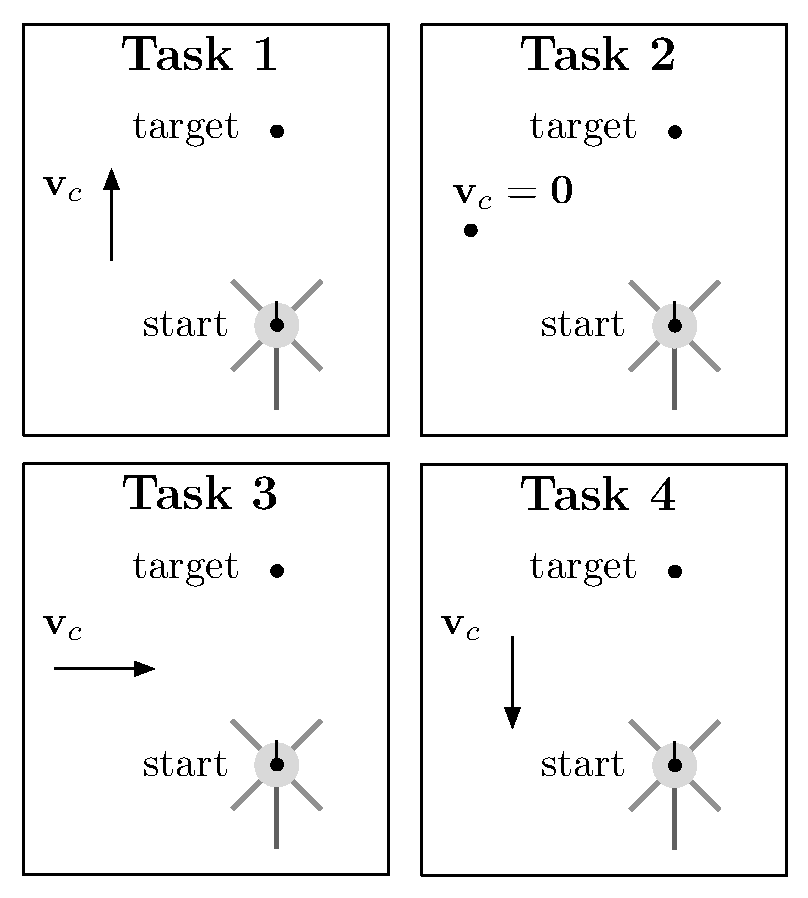
\includegraphics[scale=0.8]{fig/tasks.pdf} 
  \caption[Tasks]{\label{fig:tasks}Tasks shown in an ascending order
    of difficulty.}
\end{figure} 


\begin{comment}

  big conclusions:
   - tasks need not be easier because of morphology (if it works)
   - simpler controllers can accelerate evolution
     - hmm, I could switch between an oscillator and a CTRNN
     - maybe even if nothing is conserved between the infant and adult form
\end{comment}


This is the introduction to the thesis.\footnote{And this is a footnote.}  The conclusion is in Chapter \ref{chap:conc} on page \pageref{chap:conc}.

\section{About the logo}

Figure \ref{us_figure} shows the logo for the University of Sussex.\footnote{This is a URL: \url{http://www.sussex.ac.uk}} This is consistent with Special Relativity \citep{Einstein1905}. $E=mc^2$.

\begin{figure}
\centering

\includegraphics[width=5cm]{fig/uslogo.pdf}
\caption[US Logo (optional short caption)]{\label{us_figure} The logo for the University of Sussex.}
\end{figure}


%-----------------------------------------------------
% Chapter: Conclusion
%-----------------------------------------------------
\chapter{Conclusion}
\label{chap:conc}

I was right all along.

\section{What was I right about?}

I was right about the following things.

\subsection{Previous theories were wrong}

People thought they understood, but they didn't.

\subsection{My new idea is right}

Of course.


%%%%%%%%%%%%%%%%%%%%%%%%%%%%
% BIBLIOGRAPHY
\clearpage
\phantomsection
\addcontentsline{toc}{chapter}{Bibliography}
\bibliography{bib}
%%%%%%%%%%%%%%%%%%%%%%%%%%%%


%%%%%%%%%%%%%%%%%%%%%%%%%%%%
% START APPENDICES
\appendix
%%%%%%%%%%%%%%%%%%%%%%%%%%%%

%\include{physeqs}





%-----------------------------------------------------
% Appendix: Code
%-----------------------------------------------------
\chapter{Code}
\label{app:code}

\section{Physical Model} \label{app:code:physmod}

The equations of motion were derived using the Autolev
tool\cite{autolev}.  The source code is provided below.

%\verbatiminput[8pt]{../src/frog.al} 
\lstset{basicstyle=\scriptsize, stepnumber=9, caption=frog.al, numbers=left}
\lstinputlisting{../src/frog.al}

\subsection{Equations of Motion} \label{physeqs-sec}

\lstset{language=Mathematica, basicstyle=\scriptsize, stepnumber=9, caption=frog.al, numbers=left}
\lstinputlisting{frog_eqns_wrapped.txt} 

\subsection{Morphological Change Values} \label{morph-regiment-values}

%\begin{verbatim}
%10 PRINT "HELLO WORLD"
%\end{verbatim}


%%%%%%%%%%%%%%%%%%%%%%%%%%%%
% END DOCUMENT
\end{document}
%%%%%%%%%%%%%%%%%%%%%%%%%%%%
